% Options for packages loaded elsewhere
\PassOptionsToPackage{unicode}{hyperref}
\PassOptionsToPackage{hyphens}{url}
%
\documentclass[
  ignorenonframetext,
  aspectratio=169]{beamer}
\usepackage{pgfpages}
\setbeamertemplate{caption}[numbered]
\setbeamertemplate{caption label separator}{: }
\setbeamercolor{caption name}{fg=normal text.fg}
\beamertemplatenavigationsymbolsempty
% Prevent slide breaks in the middle of a paragraph
\widowpenalties 1 10000
\raggedbottom
\setbeamertemplate{part page}{
  \centering
  \begin{beamercolorbox}[sep=16pt,center]{part title}
    \usebeamerfont{part title}\insertpart\par
  \end{beamercolorbox}
}
\setbeamertemplate{section page}{
  \centering
  \begin{beamercolorbox}[sep=12pt,center]{part title}
    \usebeamerfont{section title}\insertsection\par
  \end{beamercolorbox}
}
\setbeamertemplate{subsection page}{
  \centering
  \begin{beamercolorbox}[sep=8pt,center]{part title}
    \usebeamerfont{subsection title}\insertsubsection\par
  \end{beamercolorbox}
}
\AtBeginPart{
  \frame{\partpage}
}
\AtBeginSection{
  \ifbibliography
  \else
    \frame{\sectionpage}
  \fi
}
\AtBeginSubsection{
  \frame{\subsectionpage}
}
\usepackage{lmodern}
\usepackage{amsmath}
\usepackage{ifxetex,ifluatex}
\ifnum 0\ifxetex 1\fi\ifluatex 1\fi=0 % if pdftex
  \usepackage[T1]{fontenc}
  \usepackage[utf8]{inputenc}
  \usepackage{textcomp} % provide euro and other symbols
  \usepackage{amssymb}
\else % if luatex or xetex
  \usepackage{unicode-math}
  \defaultfontfeatures{Scale=MatchLowercase}
  \defaultfontfeatures[\rmfamily]{Ligatures=TeX,Scale=1}
\fi
% Use upquote if available, for straight quotes in verbatim environments
\IfFileExists{upquote.sty}{\usepackage{upquote}}{}
\IfFileExists{microtype.sty}{% use microtype if available
  \usepackage[]{microtype}
  \UseMicrotypeSet[protrusion]{basicmath} % disable protrusion for tt fonts
}{}
\makeatletter
\@ifundefined{KOMAClassName}{% if non-KOMA class
  \IfFileExists{parskip.sty}{%
    \usepackage{parskip}
  }{% else
    \setlength{\parindent}{0pt}
    \setlength{\parskip}{6pt plus 2pt minus 1pt}}
}{% if KOMA class
  \KOMAoptions{parskip=half}}
\makeatother
\usepackage{xcolor}
\IfFileExists{xurl.sty}{\usepackage{xurl}}{} % add URL line breaks if available
\IfFileExists{bookmark.sty}{\usepackage{bookmark}}{\usepackage{hyperref}}
\hypersetup{
  pdftitle={Charitable Giving, Tax Reform, and Self-selection of Tax Report: Evidence from South Korea},
  hidelinks,
  pdfcreator={LaTeX via pandoc}}
\urlstyle{same} % disable monospaced font for URLs
\newif\ifbibliography
\usepackage{longtable,booktabs}
\usepackage{calc} % for calculating minipage widths
\usepackage{caption}
% Make caption package work with longtable
\makeatletter
\def\fnum@table{\tablename~\thetable}
\makeatother
\setlength{\emergencystretch}{3em} % prevent overfull lines
\providecommand{\tightlist}{%
  \setlength{\itemsep}{0pt}\setlength{\parskip}{0pt}}
\setcounter{secnumdepth}{-\maxdimen} % remove section numbering
\setbeamertemplate{navigation symbols}{}
\setbeamertemplate{footline}[page number]

\usepackage{bookmark}
\usepackage{booktabs}
\usepackage{threeparttable}
\usepackage{threeparttablex}
\usepackage{multirow}
\usepackage{array}

\usepackage{xltxtra} 
% \usepackage{zxjatype} 
\usepackage{xeCJK}
\setCJKmainfont{ipaexm.ttf}
\setCJKsansfont{ipaexg.ttf}
\setCJKmonofont{ipaexg.ttf}

% \usepackage{zxjatype}
% \setCJKmainfont[]{Meiryo}
% \setsansfont[Scale = 1.1]{Calibri}  % or Arial (Scale = 1)
\ifluatex
  \usepackage{selnolig}  % disable illegal ligatures
\fi
\newlength{\cslhangindent}
\setlength{\cslhangindent}{1.5em}
\newlength{\csllabelwidth}
\setlength{\csllabelwidth}{3em}
\newenvironment{CSLReferences}[2] % #1 hanging-ident, #2 entry spacing
 {% don't indent paragraphs
  \setlength{\parindent}{0pt}
  % turn on hanging indent if param 1 is 1
  \ifodd #1 \everypar{\setlength{\hangindent}{\cslhangindent}}\ignorespaces\fi
  % set entry spacing
  \ifnum #2 > 0
  \setlength{\parskip}{#2\baselineskip}
  \fi
 }%
 {}
\usepackage{calc}
\newcommand{\CSLBlock}[1]{#1\hfill\break}
\newcommand{\CSLLeftMargin}[1]{\parbox[t]{\csllabelwidth}{#1}}
\newcommand{\CSLRightInline}[1]{\parbox[t]{\linewidth - \csllabelwidth}{#1}\break}
\newcommand{\CSLIndent}[1]{\hspace{\cslhangindent}#1}

\title{Charitable Giving, Tax Reform, and Self-selection of Tax Report: Evidence from South Korea}
\author{true \and true \and true}
\date{2021/07/21}

\begin{document}
\frame{\titlepage}

\hypertarget{introduction}{%
\section{Introduction}\label{introduction}}

\begin{frame}{Charitable Giving and Taxiation}
\protect\hypertarget{charitable-giving-and-taxiation}{}
In many countries, governments set a tax relief for charitable giving.

To evaluate the effect of tax relief, many papers investigate the elasticity of charitable donations with respect to their tax price (Almunia et al., 2020; Auten et al., 2002; Bakija and Heim, 2011; Fack and Landais, 2010; Randolph, 1995).

Focusing on the tax deduction or tax credit on the charity, they show that the price elasticity of giving is about -1 or more in terms of absolute value.
\end{frame}

\begin{frame}{Charitable Giving and Taxiation}
\protect\hypertarget{charitable-giving-and-taxiation-1}{}
In addition to the tax price charitable donations, the donations may be affected by people's perception towards the government.

This is because the works and missions of private charity often mirror or overlap with one of governments, and the charity is not needed if the government adequately satisfies the needs of society.

Thus, the different perception towards the government may make the different behavior for charitable giving.

We investigate the relation between tax price elasticity of charitable donations and the different perception towards the government using the South Korean dataset.
\end{frame}

\begin{frame}{Summary in short}
\protect\hypertarget{summary-in-short}{}
Our result classifies that:

\begin{itemize}
\tightlist
\item
  the price elasticity of giving in Korea is -1.07 \textasciitilde{} -1.26, which is within the range of the extant research.
\item
  the amount of donation is not different between those who regard government as inefficient and the others.
\item
  the giving price elasticity of those who regard government as inefficient is more elastic than the others. This means that those who think of government as inefficient have more willingness to donate for 1\% reduction of giving price.
\end{itemize}
\end{frame}

\begin{frame}{South Korean tax reform}
\protect\hypertarget{south-korean-tax-reform}{}
We can utilize the effect of the 2014 tax reform in the South Korea.

\begin{itemize}
\tightlist
\item
  Before 2014, tax deduction was adopted to subsidize charitable donation behavior.
\item
  After 2014, tax credit have been adopted.
\end{itemize}

The main difference is that tax credits reduce taxes directly, while tax deductions indirectly lower the tax burden by decreasing the marginal tax rate, which increases with gross income.

In addition, the dataset contains the information about perception towards the government.
\end{frame}

\begin{frame}{Related Literature}
\protect\hypertarget{related-literature}{}
This study mainly relates to the two strands of studies.

\begin{enumerate}
\tightlist
\item
  Research about tax price elasticity of charitable donations
\item
  Research about perception towards the government and donation/tax payment.
\end{enumerate}
\end{frame}

\begin{frame}{Research about tax price elasticity of charitable donations}
\protect\hypertarget{research-about-tax-price-elasticity-of-charitable-donations}{}
Papers in this strand examines the price and income elasticity of charitable donations using the tax deduction applied for donation.
The estimated price elasticities vary, but the typical one is said as -1 (Andreoni and Payne, 2013).

\begin{itemize}
\tightlist
\item
  Auten et al.(2002): -0.79\textasciitilde-1.26 (the U.S.)
\item
  Fack and Landais(2010): -0.15\textasciitilde-0.57 (France)
\item
  Bakija and Heim (2011): -0.61\textasciitilde-1.1 (the U.S.)
\item
  Duquette (2016): -2.15\textasciitilde-5.01 (the U.S.)
\item
  Almunia et al.(2020): -0.24\textasciitilde--1.5 (the U.K.)
\end{itemize}

The study in non-Western country, where the culture of donation may be different, is few.
Thus, we firstly examine the elasticity of giving in Korea.
\end{frame}

\begin{frame}{Research about perception towards the government and donation/tax payment.}
\protect\hypertarget{research-about-perception-towards-the-government-and-donationtax-payment.}{}
Experimental studies show that the giving behavior may be affected by perception towards the government.

\begin{itemize}
\tightlist
\item
  Li et al.(2011) suggest that governmental organizations collect less donation than private charities though they have the same mission and work.
\item
  Sheremeta and Uler(2020) show that individuals provide public good reacting the wasteful spending of government.
\end{itemize}

This may be because people with distrust in government think that

\begin{enumerate}
\tightlist
\item
  the direct donation is more efficient than public service provision or
\item
  people can directly allocate and control their funds by donation, unlike public service provision.
\end{enumerate}

Thus, people having the different trust in the government would have different elasticities of giving.
\end{frame}

\hypertarget{institutional-background}{%
\section{Institutional background}\label{institutional-background}}

\begin{frame}{Tax relief for charitable giving by tax deduction and tax credit}
\protect\hypertarget{tax-relief-for-charitable-giving-by-tax-deduction-and-tax-credit}{}
In the South Korea, the tax policy about charitable giving drastically changed in 2014. Before then, tax relief of charitable giving was provided by tax deduction while, from 2014, tax relief by tax credit was introduced instead of tax deduction.

The tax deduction and tax credit may have different effects on giving behavior.
This section summarize the difference of tax deduction and tax credit.
\end{frame}

\begin{frame}{Budget Set}
\protect\hypertarget{budget-set}{}
Consider that a household has a choice between private consumptions (\(x_i\)) and charitable giving (\(g_i\)). Let \(y_i\) be pre-tax total income.
Then, the budget constraint is

\[
    x_i + g_i = y_i - T_i(y_i, g_i).
\]
\(T_i\) is tax amount which depends on the pre-tax income and charitable giving.
\end{frame}

\begin{frame}{Tax Deduction}
\protect\hypertarget{tax-deduction}{}
Tax deduction reduces taxable income by giving, that is,

\[
    T_i = \tau(y_i - g_i) \cdot (y_i - g_i),
\]

where \(\tau(\cdot)\) is the marginal income tax rate which is determined by \(y_i - g_i\). The budget constraint will be

\[
    x_i + [1 - \tau(y_i - g_i)]g_i = [1 - \tau(y_i - g_i)] y_i.
\]

The relative price of giving is \(p_i^{d} \equiv 1 - \tau(y_i - g_i)\).
Since the giving price in tax deduction scheme varies depending on (1) the income level and (2) the amount of charitable giving, it is endogenous to them.
\end{frame}

\begin{frame}{Tax Credit}
\protect\hypertarget{tax-credit}{}
Tax credit reduces tax amount directly, that is,

\[
    T_i = \tau(y_i)\cdot y_i - m g_i,
\]

where \(m \in [0, 1]\) is the tax credit rate. Under the tax credit system, the budget constraint is

\[
    x_i + (1 - m) g_i = [1 - \tau(y_i)] y_i.
\]

The relative price of giving is \(p_i^c = 1 - m\),
which is only dependent on the tax credit rate \(m\), which is exogenously determined by the government.
\end{frame}

\begin{frame}{Korean tax reform in 2014}
\protect\hypertarget{korean-tax-reform-in-2014}{}
\begin{itemize}
\tightlist
\item
  The tax incentives for charitable giving in Korea stared in 2000 and the market of charitable giving in Korea totaled 10.9 trillion KRW (approximately 1.09 bilion USD, 0.761\% of GDP) in 2012 according to the national tax statistics.
\item
  Since the income tax deduction was initially used as a tax incentive and the marginal income tax rate was determined as Table \ref{tab:tabTaxRate}, the minimum giving price before 2014 was 0.62.
\end{itemize}
\end{frame}

\begin{frame}{Marginal income tax rate}
\protect\hypertarget{marginal-income-tax-rate}{}
\begin{table}

\caption{\label{tab:tabTaxRate}Marginal Income Tax Rate}
\centering
\fontsize{7}{9}\selectfont
\begin{threeparttable}
\begin{tabular}[t]{lccccccc}
\toprule
Income/Year & 2008 & 2009 & 2010 \textasciitilde{} 2011 & 2012 \textasciitilde{} 2013 & 2014 \textasciitilde{} 2016 & 2017 & 2018\\
\midrule
(A) \textasciitilde{} 1200 & 8\% & 6\% & 6\% & 6\% & 6\% & 6\% & 6\%\\
\cmidrule{1-8}
(B) 1200 \textasciitilde{} 4600 & 17\% & 16\% & 15\% & 15\% & 15\% & 15\% & 15\%\\
\cmidrule{1-8}
(C) 4600 \textasciitilde{} 8800 & 26\% & 25\% & 24\% & 24\% & 24\% & 24\% & 24\%\\
\cmidrule{1-8}
(D) 8800 \textasciitilde{} 15000 &  &  &  &  & 35\% &  & 35\%\\
\cmidrule{1-1}
\cmidrule{6-6}
\cmidrule{8-8}
(E) 15000 \textasciitilde{} 30000 &  &  &  & \multirow{-2}{*}{\centering\arraybackslash 35\%} &  & \multirow{-2}{*}{\centering\arraybackslash 35\%} & 38\%\\
\cmidrule{1-1}
\cmidrule{5-5}
\cmidrule{7-8}
(F) 30000 \textasciitilde{} 50000 &  &  &  &  &  & 38\% & 40\%\\
\cmidrule{1-1}
\cmidrule{7-8}
(G) 50000 \textasciitilde{} & \multirow{-4}{*}{\centering\arraybackslash 35\%} & \multirow{-4}{*}{\centering\arraybackslash 35\%} & \multirow{-4}{*}{\centering\arraybackslash 35\%} & \multirow{-2}{*}{\centering\arraybackslash 38\%} & \multirow{-3}{*}{\centering\arraybackslash 38\%} & 40\% & 42\%\\
\bottomrule
\end{tabular}
\begin{tablenotes}
\item Notes: Marginal income tax rates applied from 2008 to 2018 are summarized. The income level is shown in terms of 10,000 KRW, which is approximately 10 United States dollars (USD) at an exchange rate of 1,000 KRW to one USD.
\end{tablenotes}
\end{threeparttable}
\end{table}
\end{frame}

\hypertarget{data}{%
\section{Data}\label{data}}

\begin{frame}{National Survey of Tax and Benefit (NaSTaB)}
\protect\hypertarget{national-survey-of-tax-and-benefit-nastab}{}
\begin{itemize}
\tightlist
\item
  An annual financial panel survey implemented by The Korea Institute of Taxation and Finance implements to study the tax burden of households and the benefits that households receive from government.
\item
  The subjects of this survey are general household and household members living in 15 cities and provinces nationwide.
\item
  This survey is based on a face-to-face interview. If it is difficult for investigators to meet subjects, another family member answers on behalf of him.
\item
  We use data from 2012 to 2018 \textbf{since the items of the value survey which we focused is not available before 2012 (ここは違いま???)}. In addition, we exclude the subject of the sample, whose age is under 23, since they are not likely to have income or asset.
\end{itemize}
\end{frame}

\begin{frame}{Summary Statistics}
\protect\hypertarget{summary-statistics}{}
\begin{table}
\centering\begingroup\fontsize{7}{9}\selectfont

\begin{tabular}{lcccccc}
\toprule
 & N & Mean & Std.Dev. & Min & Median & Max\\
\midrule
\addlinespace[0.3em]
\multicolumn{7}{l}{\textbf{Charitable Donations}}\\
\hspace{1em}Annual charitable giving (unit: 10,000KRW) & 67848 & 29.52 & 132.91 & 0.00 & 0.00 & 10000.00\\
\hspace{1em}Dummy of Donation > 0 & 67848 & 0.20 & 0.40 & 0.00 & 0.00 & 1.00\\
\addlinespace[0.3em]
\multicolumn{7}{l}{\textbf{Income, giving price, and tax report}}\\
\hspace{1em}Annual taxable income (unit: 10,000KRW) & 53269 & 1876.12 & 2700.97 & 0.00 & 900.00 & 91772.00\\
\hspace{1em}First giving price & 62877 & 0.86 & 0.04 & 0.62 & 0.85 & 0.94\\
\hspace{1em}Dummy of tax report & 18596 & 0.30 & 0.46 & 0.00 & 0.00 & 1.00\\
\addlinespace[0.3em]
\multicolumn{7}{l}{\textbf{Individual Characteristics}}\\
\hspace{1em}Age & 67848 & 51.35 & 15.81 & 24.00 & 50.00 & 104.00\\
\hspace{1em}Female dummy & 67848 & 0.53 & 0.50 & 0.00 & 1.00 & 1.00\\
\hspace{1em}Employee dummy & 42362 & 0.53 & 0.50 & 0.00 & 1.00 & 1.00\\
\hspace{1em}University graduate & 67842 & 0.41 & 0.49 & 0.00 & 0.00 & 1.00\\
\hspace{1em}High school graduate dummy & 67842 & 0.35 & 0.48 & 0.00 & 0.00 & 1.00\\
\hspace{1em}Junior high school graduate dummy & 67842 & 0.24 & 0.43 & 0.00 & 0.00 & 1.00\\
\bottomrule
\end{tabular}
\endgroup{}
\end{table}
\end{frame}

\begin{frame}{Charitable Giving}
\protect\hypertarget{charitable-giving}{}
\begin{figure}[t]

{\centering 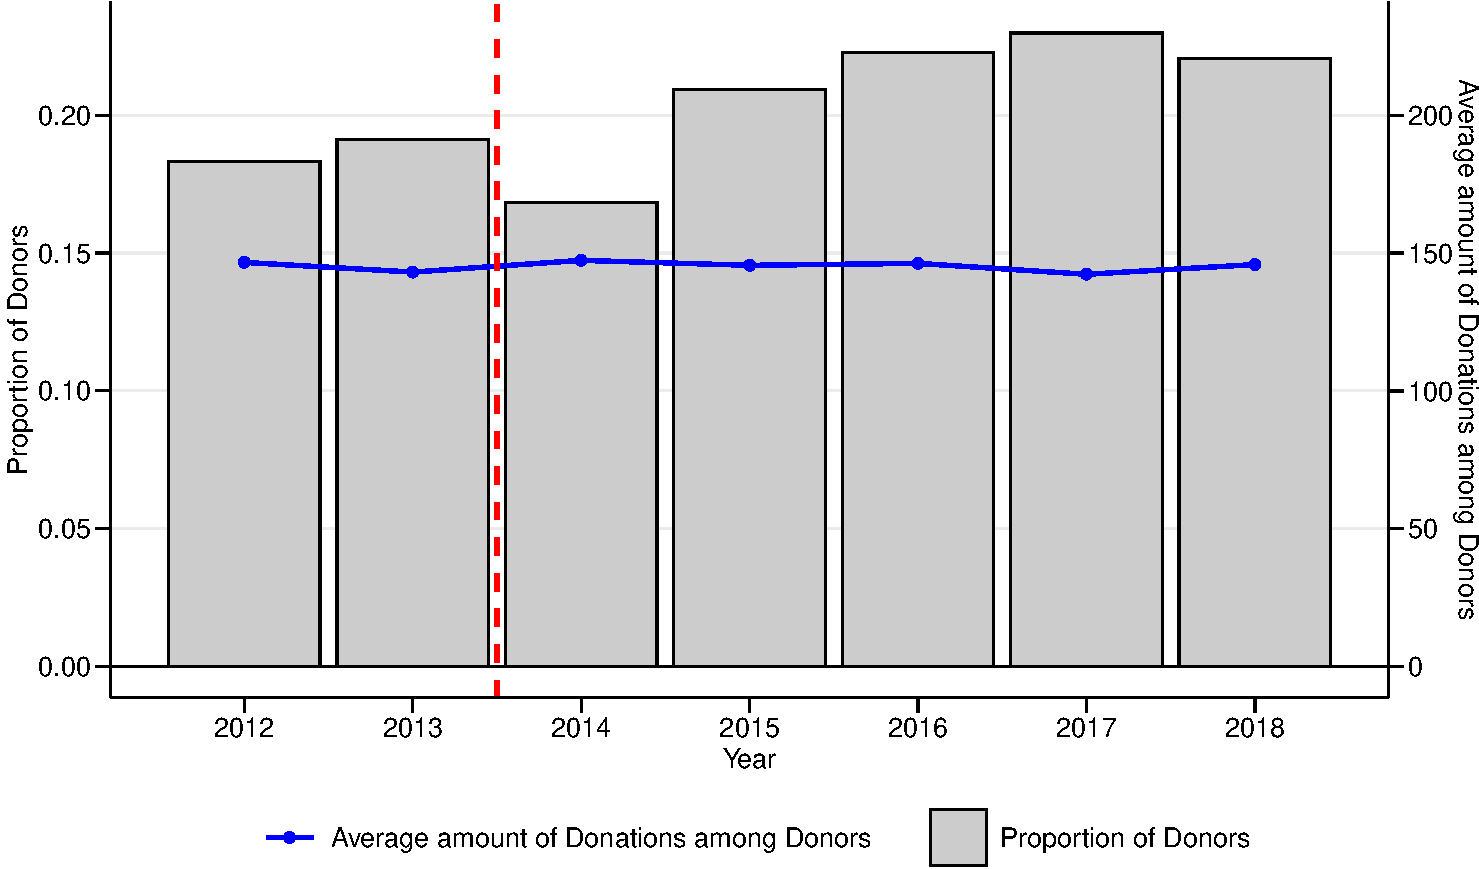
\includegraphics[width=0.9\linewidth]{C:/Users/katoo/Desktop/NASTAB/paper/slide_files/figure-beamer/SummaryOutcome-1} 

}

\caption{Proportion of Donors and Average Donations among Donors. Notes: The left and right axises respectively mesure proportion of donors and the average amount donations among donors. Authors made this graph based on NasTaB data.}\label{fig:SummaryOutcome}
\end{figure}
\end{frame}

\begin{frame}{Income and Giving Price}
\protect\hypertarget{income-and-giving-price}{}
\begin{itemize}
\tightlist
\item
  Figure \ref{fig:showSummaryPriceChange} shows the giving price after 2012 and income distribution in 2013.

  \begin{itemize}
  \tightlist
  \item
    Blue line shows the giving price in 2012 and 2013, which depends on income
  \item
    Red dashed line shows the giving price after 2014, which is not a function of income.
  \end{itemize}
\item
  We can make three groups in terms of the benefit from the 2014 tax reform.

  \begin{itemize}
  \tightlist
  \item
    Benefit group: Final taxable income is less than \(1200 \times 10^4\)KRW.
  \item
    Neutral group: Final taxable income lies between \((1200 \times 10^4, 4600 \times 10^4)\).
  \item
    Loss group: Final taxable income is more than \(4600 \times 10^4\)KRW.
  \end{itemize}
\end{itemize}
\end{frame}

\begin{frame}{Giving Price and Income Distribution (Cont'd)}
\protect\hypertarget{giving-price-and-income-distribution-contd}{}
\begin{figure}[t]

{\centering 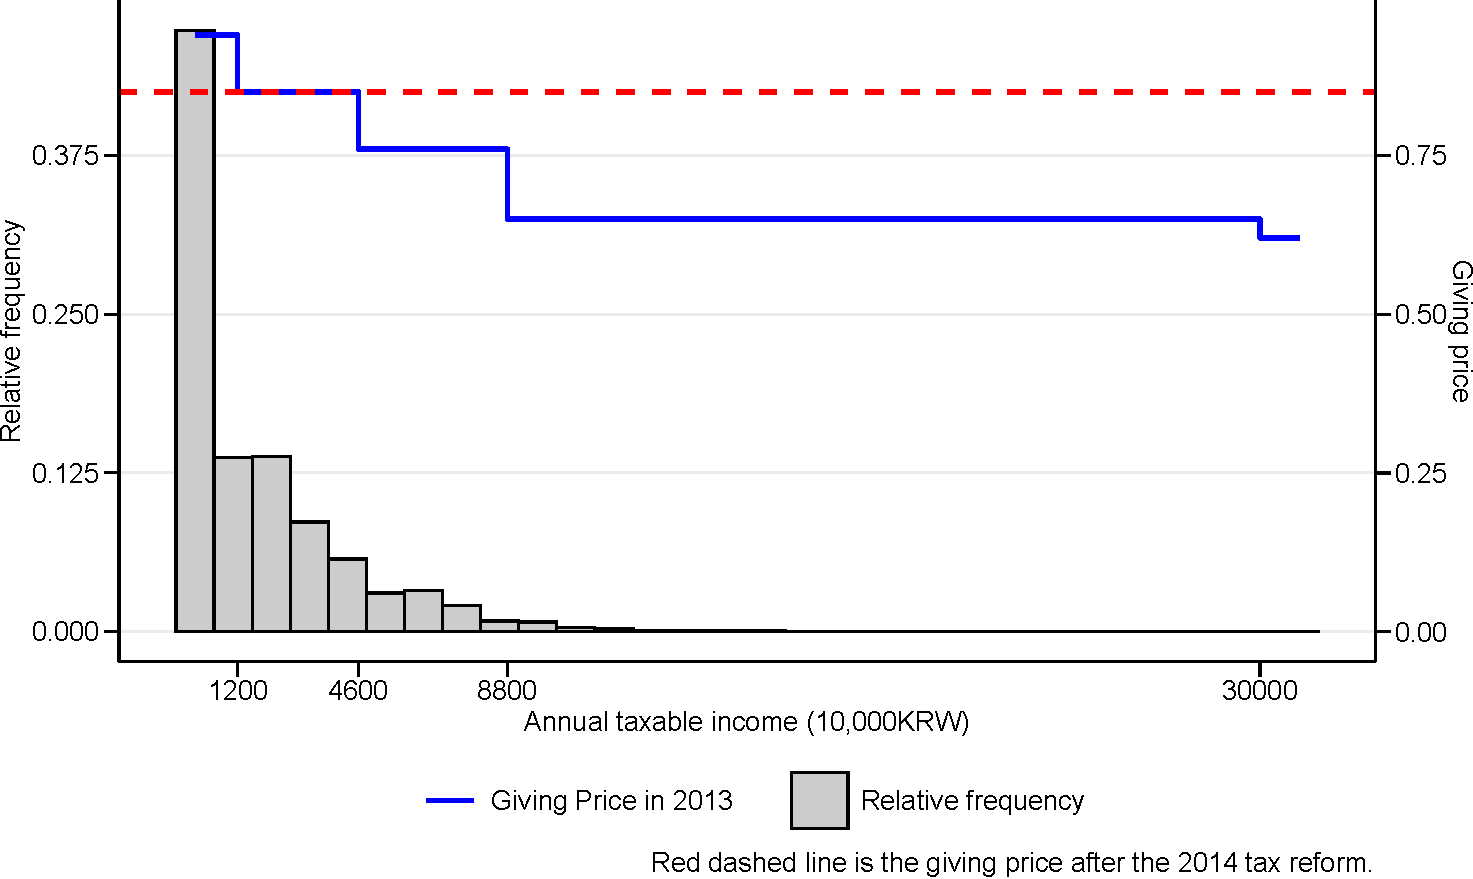
\includegraphics[width=0.9\linewidth]{C:/Users/katoo/Desktop/NASTAB/paper/slide_files/figure-beamer/SummaryPriceChange-1} 

}

\caption{Income Distribution and Giving Price in 2013}\label{fig:SummaryPriceChange}
\end{figure}

\clearpage
\end{frame}

\hypertarget{references}{%
\section*{References}\label{references}}
\addcontentsline{toc}{section}{References}

\begin{frame}[allowframebreaks]{References}
\hypertarget{refs}{}
\begin{CSLReferences}{1}{0}
\leavevmode\hypertarget{ref-Almunia2020}{}%
Almunia, M., Guceri, I., Lockwood, B., Scharf, K., 2020. More giving or more givers? The effects of tax incentives on charitable donations in the UK. Journal of Public Economics 183. doi:\href{https://doi.org/10.1016/j.jpubeco.2019.104114}{10.1016/j.jpubeco.2019.104114}

\leavevmode\hypertarget{ref-Auten2002}{}%
Auten, G.E., Sieg, H., Clotfelter, C.T., 2002. Charitable giving, income, and taxes: An analysis of panel data. American Economic Review 92, 371--382.

\leavevmode\hypertarget{ref-Bakija2011}{}%
Bakija, J., Heim, B.T., 2011. How does charitable giving respond to incentives and income? New estimates from panel data. National Tax Journal 64, 615--650. doi:\href{https://doi.org/10.17310/ntj.2011.2S.08}{10.17310/ntj.2011.2S.08}

\leavevmode\hypertarget{ref-Fack2010}{}%
Fack, G., Landais, C., 2010. Are tax incentives for charitable giving efficient? Evidence from france. American Economic Journal - Economic Policy 2, 117--141. doi:\href{https://doi.org/10.1257/pol.2.2.117}{10.1257/pol.2.2.117}

\leavevmode\hypertarget{ref-Randolph1995}{}%
Randolph, W.C., 1995. Dynamic income, progressive taxes, and the timing of charitable contributions. Journal of Political Economy 103, 709--738. doi:\href{https://doi.org/10.1086/262000}{10.1086/262000}

\end{CSLReferences}
\end{frame}

\end{document}
